\PassOptionsToPackage{xetex}{xcolor}
\PassOptionsToPackage{xetex}{graphicx}
\documentclass[a4paper,landscape,headrule,footrule,xetex]{foils}

%%
%%%  Macros
%%%
\newcommand{\logo}{~}
\MyLogo{HG2052 (2020)}
%\newcommand{\Story}{\SHA{HOUN}{The Hound of the Baskervilles}}

\newcommand{\header}[3]{%
\title{\vspace*{-2ex} \Large HG2052
\\\large  Language, Technology and the Internet
\\[2ex] \Large  \emp{#2}}
\author{\blu{Francis Bond}   \\ 
\normalsize  \textbf{Division of Linguistics and Multilingual Studies}\\
\normalsize  \url{http://www3.ntu.edu.sg/home/fcbond/}\\
\normalsize  \texttt{bond@ieee.org}}
\MyLogo{HG2052 (2020)}
\date{#1}
\renewcommand{\logo}{#2}
 \hypersetup{
   pdfinfo={
     Author={Francis Bond},
     Title={#1: #2},
     Subject={HG2052: Language, Technology and the Internet},
     Keywords={Language, Technology, Internet},
     License={CC BY 4.0}
   }
 %  pdfcopyright={Copyright © Francis Bond. Creative Commons 4.0 Attribution License.}
 %  pdflicenseurl={http://creativecommons.org/licenses/by/4.0/}
 }
}


%%
%% Multilingual Stuff
%%
\usepackage[a4paper,landscape,margin=25mm]{geometry}

\usepackage{fontenc}
\usepackage{polyglossia}
\setmainlanguage{english}
\setmainfont{TeX Gyre Pagella}
%\setmainfont{Linux Libertine}
%\setmainfont{Charis SIL}
\newfontfamily{\ipafont}{Gentium}
\newcommand{\ipa}[1]{{\ipafont\selectfont #1}}
\usepackage{xeCJK}

\setCJKmainfont{Noto Sans CJK SC}
\setCJKsansfont{Noto Sans CJK SC}
%\setCJKttfont{Noto Sans CJK SC}
%\setCJKmainfont{WenQuanYi Micro Hei}
%\clearpage
%\setCJKmainfont{AR PL SungtiL GB}

\usepackage[xetex]{xcolor}
\usepackage[xetex]{graphicx}
\newcommand{\blu}[1]{\textcolor{blue}{#1}}
\newcommand{\grn}[1]{\textcolor{green}{#1}}
\newcommand{\hide}[1]{\textcolor{white}{#1}}
\newcommand{\emp}[1]{\textcolor{red}{#1}}
\newcommand{\txx}[1]{\textbf{\textcolor{blue}{#1}}}
\newcommand{\lex}[1]{\textbf{\mtcitestyle{#1}}}

\usepackage{pifont}
\renewcommand{\labelitemi}{\textcolor{violet}{\ding{227}}}
\renewcommand{\labelitemii}{\textcolor{purple}{\ding{226}}}

\newcommand{\subhead}[1]{\noindent\textbf{#1}\\[5mm]}

\newcommand{\Bad}{\emp{\raisebox{0.15ex}{\ensuremath{\mathbf{\otimes}}}}}
\newcommand{\bad}{*}

\newcommand{\com}[1]{\hfill \textnormal{(\emp{#1})}}%
\newcommand{\cxm}[1]{\hfill \textnormal{(\txx{#1})}}%
\newcommand{\cmm}[1]{\hfill \textnormal{(#1)}}%
\usepackage{amssymb}
\usepackage{relsize,xspace}
\newcommand{\into}{\ensuremath{\rightarrow}\xspace}
\newcommand{\ent}{\ensuremath{\Rightarrow}\xspace}
\newcommand{\nent}{\ensuremath{\not\Rightarrow}\xspace}
\newcommand{\tot}{\ensuremath{\leftrightarrow}\xspace}
\usepackage{url}
\usepackage[hidelinks]{hyperref}
\hypersetup{
     colorlinks,
     linkcolor={blue!50!black},
     citecolor={red!50!black},
     urlcolor={blue!80!black}
}
%\usepackage{hyperxmp}
\usepackage{url}
\newcommand{\lurl}[1]{\MyLogo{\url{#1}}}

\usepackage{mygb4e}
\let\eachwordone=\itshape
\newcommand{\lx}[1]{\textbf{\textit{#1}}}
\newcommand{\ix}{\ex\it}

\newcommand{\cen}[2]{\multicolumn{#1}{c}{#2}}
%\usepackage{times}
%\usepackage{nttfoilhead}
\newcommand{\myslide}[1]{%
\foilhead[-25mm]{\raisebox{12mm}[0mm]{\emp{#1}}}%
\leftheader{}%
\MyLogo{\logo}}

\newcommand{\mytask}[1]{%
\foilhead[-25mm]{\raisebox{12mm}[0mm]{\emp{#1}}}
\leftheader{🔍 Hi}%
\MyLogo{\logo}}

\newcommand{\myslider}[1]{\rotatefoilhead[-25mm]{\raisebox{12mm}[0mm]{\emp{#1}}}}
%\newcommand{\myslider}[1]{\rotatefoilhead{\raisebox{-8mm}{\emp{#1}}}}

\newcommand{\section}[1]{\myslide{}{\begin{center}\Huge \emp{#1}\end{center}}}

\usepackage{tcolorbox}
% \newcommand{\task}{\marginpar{\raisebox{-1ex}{\large
%       \tcbox[colframe=red,colback=white,arc=3pt]{\textbf{?}}}}}
% \newcommand{\task}{\marginpar{\raisebox{-1ex}{
%       \hspace{-0.5em}\tcbox[colframe=red,colback=white,arc=3pt]{%
%         \includegraphics[width=1.5em]{pics/detective}}}}}
\newcommand{\task}{\marginpar{\raisebox{-2ex}{
      \hspace{-0.5em}\reflectbox{\includegraphics[width=2em]{pics/detective}}}}}

\usepackage[lyons,j,e,k]{mtg2e}
\renewcommand{\mtcitestyle}[1]{\textcolor{teal}{\textsl{#1}}}
%\renewcommand{\mtcitestyle}[1]{\textsl{#1}}
\newcommand{\chn}{\mtciteform}
\newcommand{\cmn}{\mtciteform}
\newcommand{\iz}[1]{\textup{\texttt{\textcolor{blue}{\textbf{#1}}}}}
\newcommand{\con}[1]{\textsc{#1}}
\newcommand{\gm}{\textsc}
\newcommand{\cmp}[1]{{[\textsc{#1}]}}
\newcommand{\sr}[1]{\ensuremath{\langle}#1\ensuremath{\rangle}}
\usepackage[normalem]{ulem}
\newcommand{\ul}{\uline}
\newcommand{\uul}{\uuline}
\newcommand{\wl}{\uwave}
\newcommand{\vs}{\ensuremath{\Leftrightarrow}~}
%%%
%%% Bibliography
%%%
\usepackage{natbib}
%\usepackage{url}
\usepackage{bibentry}


%%% From Tim
\newcommand{\WMngram}[1][]{$n$-gram#1\xspace}
\newcommand{\infers}{$\rightarrow$\xspace}



\usepackage{rtrees,qtree}
\renewcommand{\lf}[1]{\br{#1}{}}
\usepackage{avm}
%\avmoptions{topleft,center}
\newcommand{\ft}[1]{\textsc{#1}}
\newcommand{\val}[1]{\textit{#1}}
\newcommand{\typ}[1]{\textit{#1}}
\avmfont{\sc}
%\avmvalfont{\sc}
\renewcommand{\avmtreefont}{\sc}
\avmsortfont{\it}


%%% From CSLI book
\newcommand{\mc}{\multicolumn}
\newcommand{\HD}{\textbf{H}\xspace}
\newcommand{\el}{\< \>}
\makeatother
\long\def\smalltree#1{\leavevmode{\def\\{\cr\noalign{\vskip12pt}}%
\def\mc##1##2{\multispan{##1}{\hfil##2\hfil}}%
\tabskip=1em%
\hbox{\vtop{\halign{&\hfil##\hfil\cr
#1\crcr}}}}}
\makeatletter

\newcommand{\sh}[1]{\href{https://www.arthur-conan-doyle.com/index.php?title=#1}{#1}}
\newcommand{\SHA}[2]{\href{https://www.arthur-conan-doyle.com/index.php?title=#1}{\textit{#2}}}

\newcommand{\deu}{\mtciteform}

\header{Lecture 2}{Writing as Language Technology}

\begin{document}
\bibliographystyle{apalike}
\nobibliography{abb,mtg,nlp,ling}

\maketitle

\myslide{Overview}

\begin{itemize}
\item The origins of writing %%%FIXME
\item Different writing systems
\item Representing writing on computers
\item Writing versus talking
\end{itemize}

\myslide{The Origins of Writing}
\begin{itemize}
\item Writing was invented independently in at least three places:
  \begin{itemize}
  \item Mesopotamia
  \item China
  \item Mesoamerica
  \end{itemize}
  Probably also Egypt
  (\href{https://archive.archaeology.org/9903/newsbriefs/egypt.html}{Earliest
  Egyptian Glyphs}) and possibly the Indus valley.
\item The written records are incomplete
\item Gradual development from pictures/tallies
\end{itemize}

\myslide{Follow the money}

\begin{itemize}
\item Before 2700, writing is only accounting.
  \begin{itemize}
  \item Temple and palace accounts
  \item Gold, Wheat, Sheep
  \end{itemize}
\item How it developed in Mesopotamia
  \begin{itemize}
  \item One token per thing (in a clay envelope)
  \item One token per thing in the envelope and marked on the outside
  \item One mark per thing
  \item One mark and a symbol for the number
  \item Finally symbols for names
  \end{itemize}
\end{itemize}

Denise Schmandt-Besserat (1997) \textit{How writing came about}. University of Texas Press


% The Sumerians of the Uruk period  used clay tokens to count their agricultural and manufactured foods. They would place the tokens in hollow clay containers and mark the lids with the number of tokens inside. They impressed a picture of the token inside as many times as the amount of tokens. Later they realized that they did not have to use both the tokens and the inscription on the containers, so they started using only the inscription. Later yet this system was streamlined with the introduction of symbols for numbers: for example, to avoid making 100 pictures to represent 100 tokens they started using a dedicated symbol for 100 together with a single token picture. Thus writing began.[7]

\newpage
\noindent\begin{tabular}{cc}
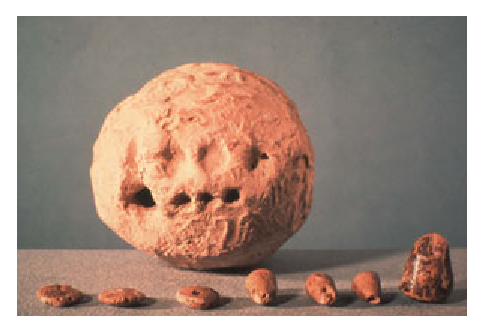
\includegraphics[width=0.6\textwidth]{../pics/clay-envelope.eps} &
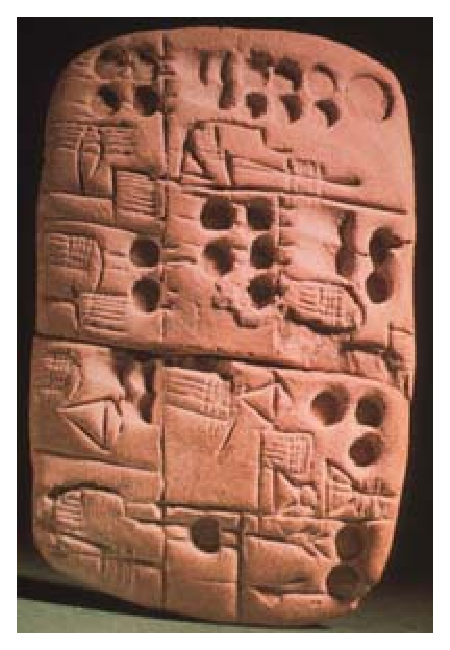
\includegraphics[height=0.9\textheight]{../pics/clay-tablet.eps} \\
Clay Tokens and Envelope & Clay Tablet\\
\end{tabular}


\myslide{Writing systems used for human languages}

\begin{itemize}
\item What is writing?
\begin{quote}
  A system of more or less permanent marks used to represent an utterance in such a way that it can be recovered more or less exactly without the intervention of the utterer.  \hfill \textit{Peter T. Daniels, The World's Writing Systems}
\end{quote}

\item Different types of writing systems are used:
\begin{itemize}
\item Alphabetic
\item Syllabic
\item Logographic
\end{itemize}
\end{itemize}





\myslide{What is represented?}
%%% FIXME
In English:
\begin{itemize}
\item Phonemes:  \ipa{/maɪ dɒg laɪks ˈɒrɪnʤɪz/} \com{45}

\item Syllables:  \ipa{maɪ dɒg laɪks (ˈɒr)(ɪn)(ʤɪz)}  \com{10,000+}
\item Morphemes:  my/me+'s dog like+s orange+s   \com{100,000+}
\item Words: \eng{my dog likes oranges} \com{200,000+}
\item Concepts: \iz{speaker poss dog$_{canine}$:SG fond orange$_{fruit}$:PL}  \com{400,000++}
\end{itemize}
\bigskip
\begin{enumerate}
\item Some languages have fewer syllables
\item It is hard to visually distinguish 1,000+ different symbols, \ldots
\end{enumerate}


\myslide{Alphabetic systems}

\begin{itemize}
\item Alphabets (phonemic alphabets)
\begin{itemize}
\item represent all sounds, i.e., consonants and vowels
\item Examples: Etruscan, Latin, Cyrillic, Runic, International Phonetic Alphabet, ?Korean 
\end{itemize}

\item Abjads (consonant alphabets)
\begin{itemize}
\item represent consonants only (sometimes plus selected vowels; vowel diacritics generally available)
\item Examples: Arabic, Aramaic, Hebrew
\end{itemize}
\end{itemize}





\myslide{Alphabet example: Russian}

The Cyrillic alphabet is used to write many languages, mainly Slavic.
Here is the set used for Russian.

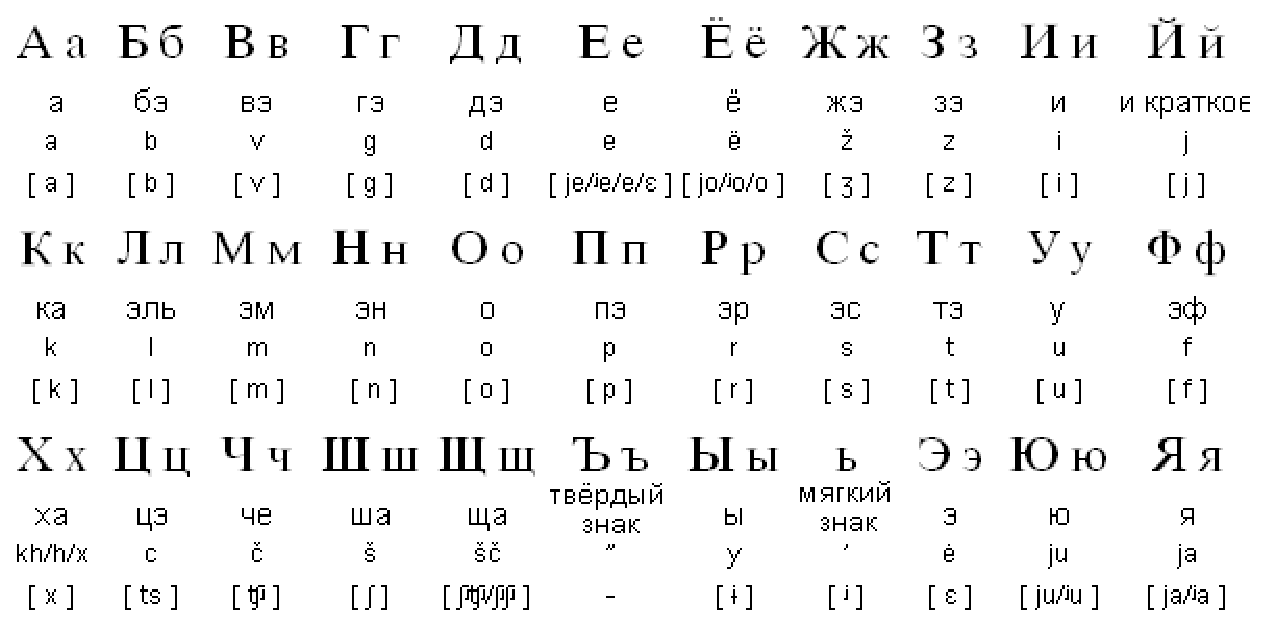
\includegraphics{../pics/russian.eps}




(from: http://www.omniglot.com/writing/russian.htm)


\myslide{Abjad example: Phoenician}

An abjad used to write Phoenician, created between the 18th and 17th
centuries BC; assumed to be the forerunner of the Greek and Hebrew
alphabet.




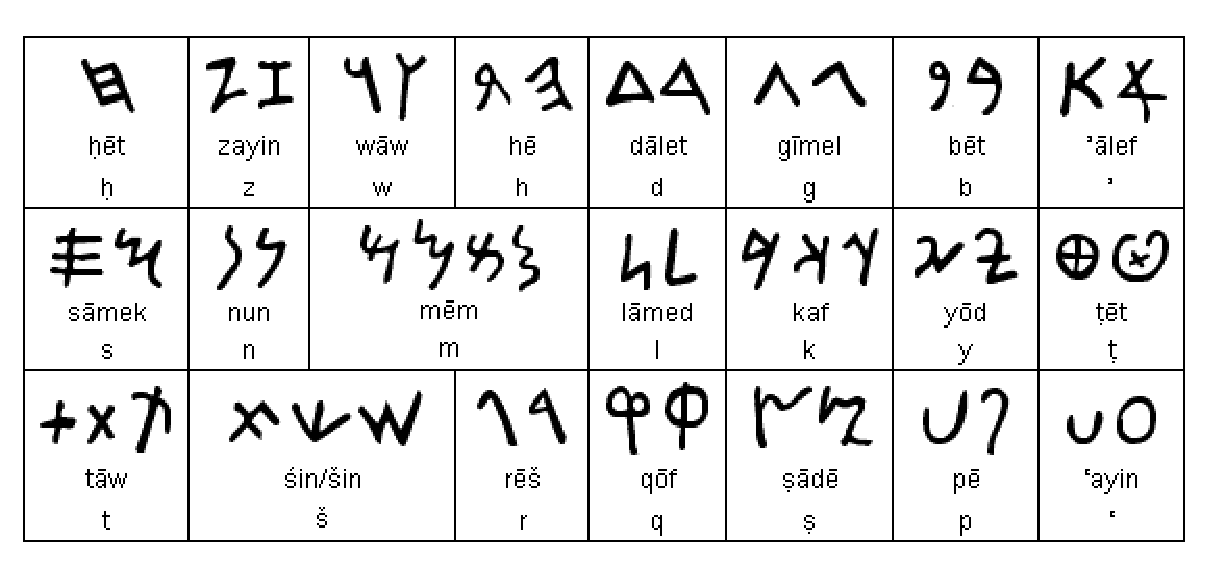
\includegraphics{../pics/phonecian.eps}



(from: \url{http://www.omniglot.com/writing/phoenician.htm})




\myslide{A note on the letter-sound correspondence}
\begin{itemize}
\item Alphabets use letters to encode sounds (consonants, vowels).
\item But the correspondence between spelling and pronounciation in many languages is quite complex, i.e., not a simple one-to-one correspondence.
\item Example: English
\begin{itemize}
\item same spelling\,–\,different sounds: \blu{ough}: \eng{ought, cough, tough, through, though, hiccough}
\item silent letters: \eng{knee, knight, knife, debt, psychology, mortgage}
\item one letter\,–\,multiple sounds: \eng{exit}
\item multiple letters\,–\,one sound: \eng{the, revolution}
\item alternate spellings: \eng{jail} or \eng{gaol}
\end{itemize}
\end{itemize}



% \myslide{More examples for non-transparent letter-sound correspondences}
% French
% (1) a. Versailles → [veRsai] b. ete, etais, etait, etaient → [ete]


% Irish
% (2) a. Baile A’tha Cliath (Dublin) → [bl’a: kli uh] b. samhradh (summer) → [sauruh] c. scri’obhaim (I write) → [shgri:m] What is the notation used within the []?

% \myslide{The International Phonetic Alphabet (IPA)}



% Several special alphabets for representing sounds have been developed, the best known being the International Phonetic Alphabet (IPA). The phonetic symbols are unambiguous:
% designed so that each speech sound gets its own symbol, eliminating the need for
% multiple symbols used to represent simple sounds one symbol being used for multiple sounds.



% Interactive example chart: http://web.uvic.ca/ling/ resources/ipa/charts/IPAlab/IPAlab.htm

\myslide{Capitalization Can Carry Meaning}
\MyLogo{\url{http://yourfuckingmuse.tumblr.com/post/18793564230/today-a-lesson-in-german-capitalisation}}
\begin{itemize}
\item 
  \begin{itemize}
  \item \deu[The spiders!]{Die Spinnen!}
  \item \deu[They are crazy!]{Die spinnen!}
  \end{itemize}
\item \begin{itemize}
  \item \deu[He had kind companions.]{Er hatte liebe Genossen.}
  \item \deu[He had enjoyed love.]{Er hatte Liebe genossen.}
  \end{itemize}
\item \begin{itemize}
  \item \deu[to gloat and turn towards other things]{Sich brüsten und Anderem zuwenden.}
  \item \deu[to turn towards breasts and other things]{Sich Brüsten und Anderem zuwenden.}
  \end{itemize}
% \item \begin{itemize}
%   \item \deu[She was adept at treating blisters and limbs.]{Sie konnte geschickt Blasen und Gliede behandeln.}
%   \item \deu[She was adept at giving blowjobs and handling members.]{Sie konnte geschickt blasen ud Glieder behandeln.}
%   \end{itemize}
\item \begin{itemize}
  \item \deu[The prisoner escaped.]{Der Gefangene floh.}
  \item \deu[The imprisoned flea]{Der gefangene Floh.}
  \end{itemize}
% \item \begin{itemize}
%   \item \deu[Help the poor birds.]{Helft den armen Vögeln.}
%   \item \deu[Help poor people with sex.]{Helft den Armen vögeln.}
%   \end{itemize}
\end{itemize}

% \myslide{Consonants and Vowels in Arabic}
% {\arabicfont
% \begin{tabular}{llllll}
%    عَقَدَ  & ‘to tie’ &  عِقْدٌ  &  ‘lace’ &  عَقُدَ  & ‘became knotty’\\
%    حُبّ &   ‘love’ &     حَبْ &  ‘grain’ &  حِبْ &  ‘love!’\\
%    شَاهَدَ  &  ‘to watch’ &  شَاهِدٌ  &  ‘witness’ &  شَاهِدْ  & ‘watch!’\\
%    خَبَّرَ  & ‘to tell’ &  خَبَرٌ  &  ‘a piece of news’ &  خَبَرَ  &  ‘to know’\\
%    خَبُرَ  &  ‘to become an expert’ &  خَبِرٌ &  ‘familiar with’ &  خَبَرَ  &  ‘to plough’\\
% \end{tabular}}


\myslide{Syllabic systems}
\MyLogo{}
\begin{itemize}
\item Syllabic alphabets (Alphasyllabaries)
\begin{itemize}
\item writing systems with symbols that represent a consonant with a
  vowel, but the vowel can be changed by adding a diacritic (= a
  symbol added to the letter).
\item Examples: Balinese, Javanese, Tibetan, Tamil, Thai, Tagalog
\end{itemize}
\item Syllabaries
\begin{itemize}
\item writing systems with separate symbols for each syllable of a language
\item Examples: Cherokee. Ethiopic, Cypriot, Ojibwe, Hiragana (Japanese)
\end{itemize}
\end{itemize}





% \myslide{Syllabary example: Cypriot}

% The Cypriot syllabary or Cypro-Minoan writing is thought to have
% developed from the Linear A, or possibly the Linear B script of Crete,
% though its exact origins are not known. It was used from about 800 to
% 200 BC.
% (from: http://www.omniglot.com/writing/cypriot.htm)


\myslide{Syllabic alphabet example: Lao} Script developed in the 14th
century to write the Lao language, based on an early version of the
Thai script, which was developed from the Old Khmer script, which was
itself based on Mon scripts.

Example for vowel diacritics around the letter k:

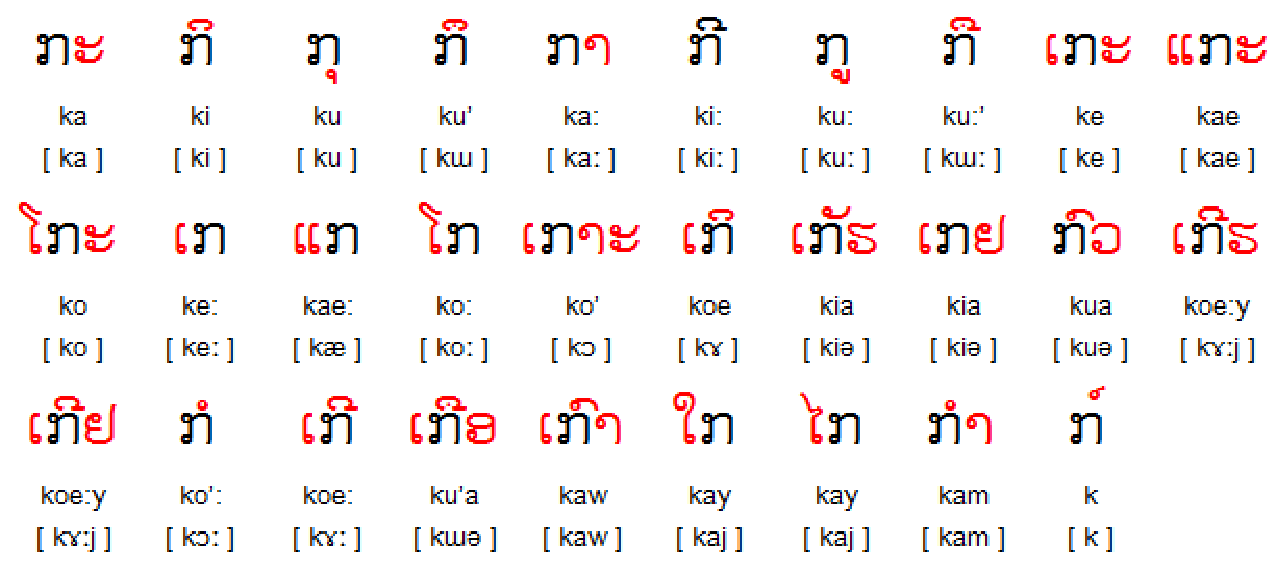
\includegraphics{../pics/lao_vwl.eps}

% (from: \url{http://www.omniglot.com/writing/lao.htm})

\myslide{Syllabic alphabet example: Hiragana} 
Script developed in 10th century from Chinese characters. 52 characters.

%Hiragana were originally called onnade or 'women's hand' as were used
%mainly by women - men wrote in kanji and katakana. By the 10th
%century, hiragana were used by everybody.
\begin{center}
  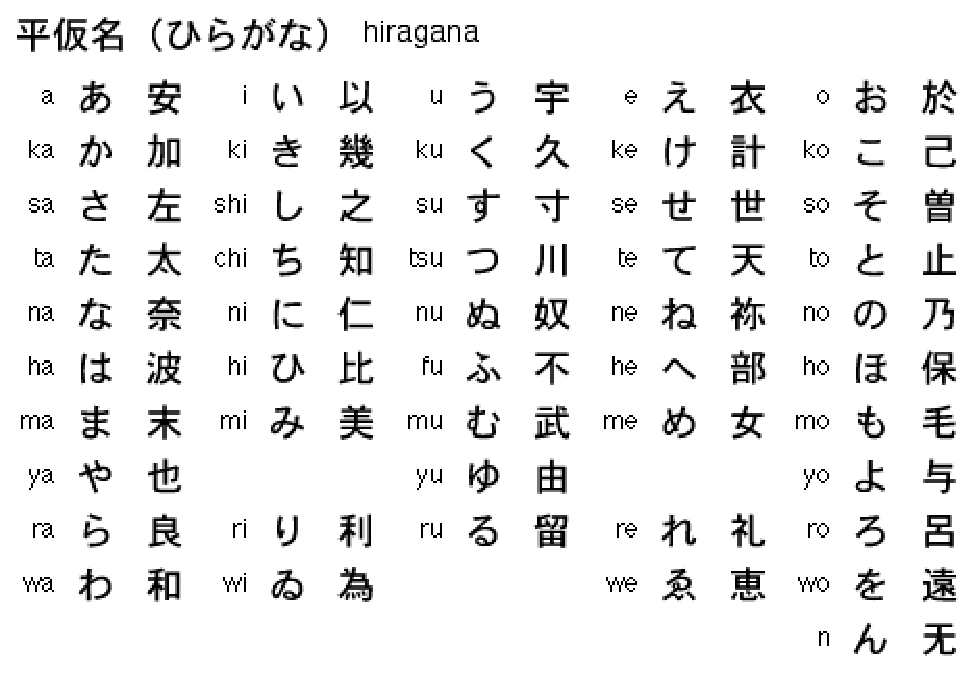
\includegraphics{../pics/hiragana.eps}
\end{center}
\myslide{Logographic writing systems}
\begin{itemize}
\item Logographs (also called Logograms):
\begin{itemize}
\item Pictographs (Pictograms): originally pictures of things, now stylized and simplified.
\item Ideographs (Ideograms): representations of abstract ideas
\item Compounds: combinations of two or more logographs.
\item Semantic-phonetic compounds: symbols with a meaning element (hints at meaning) and a phonetic element (hints at pronunciation).
\end{itemize}

\item Examples: Chinese (Japanese, Vietnamese), Mayan, Ancient Egyptian
\end{itemize}

\myslide{Development of Chinese character horse}

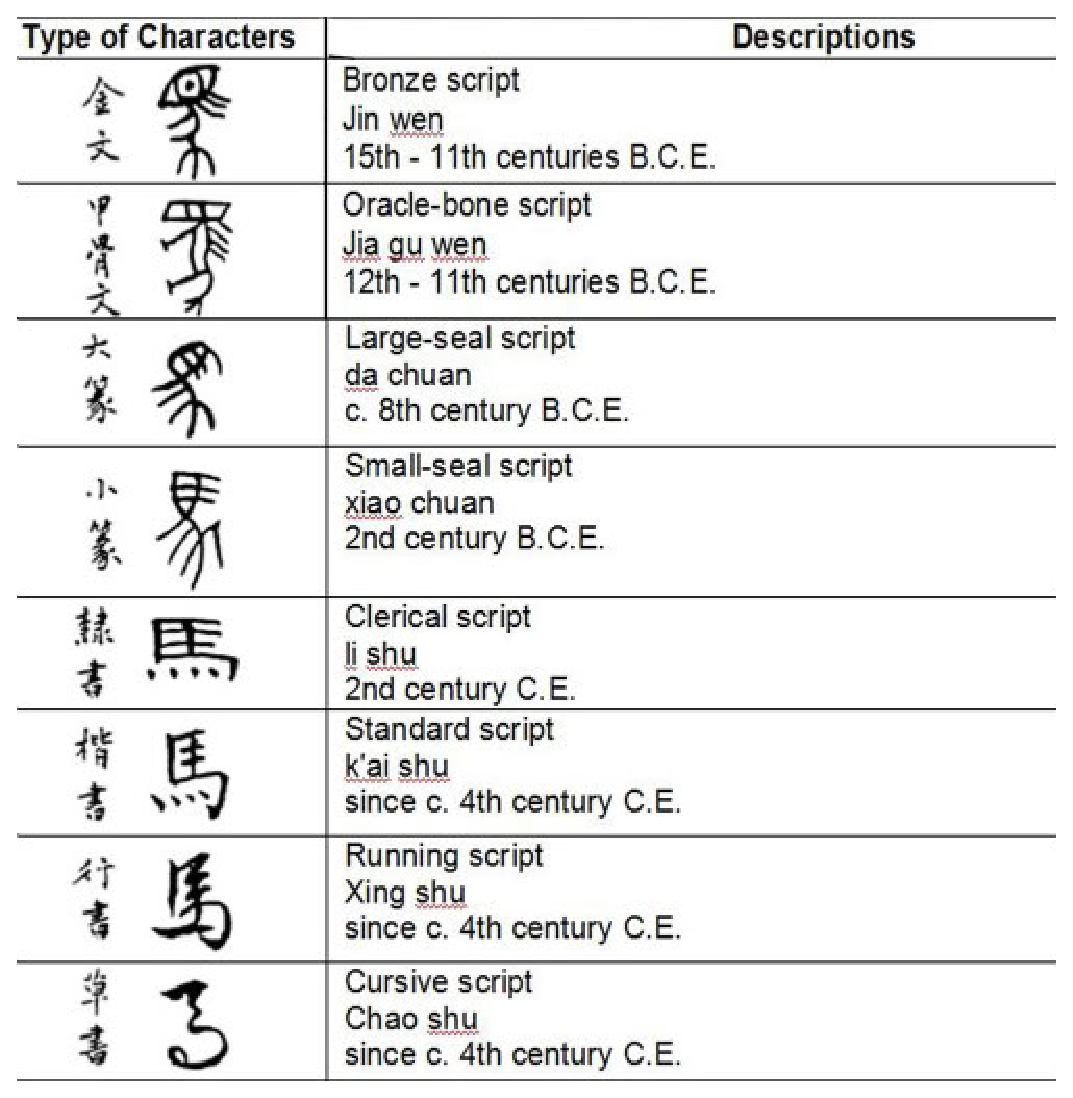
\includegraphics[height=\textheight]{../pics/horse-hanzi.eps}


\myslide{Logograph writing system example: Chinese}
\begin{itemize}
\item Pictographs\\
  
\includegraphics{../pics/hanzi-1.eps}
\item Ideographs\\
  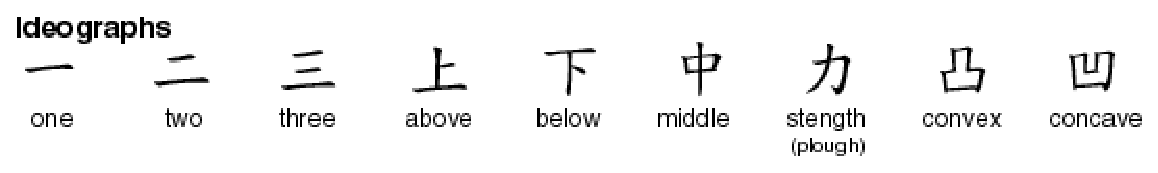
\includegraphics{../pics/hanzi-2.eps}
\item Compounds of Pictographs/Ideographs\\
  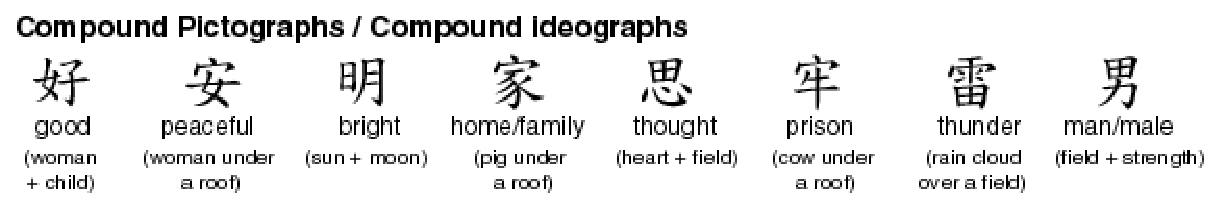
\includegraphics{../pics/hanzi-3.eps}
\end{itemize}


\myslide{Semantic-phonetic compounds}

 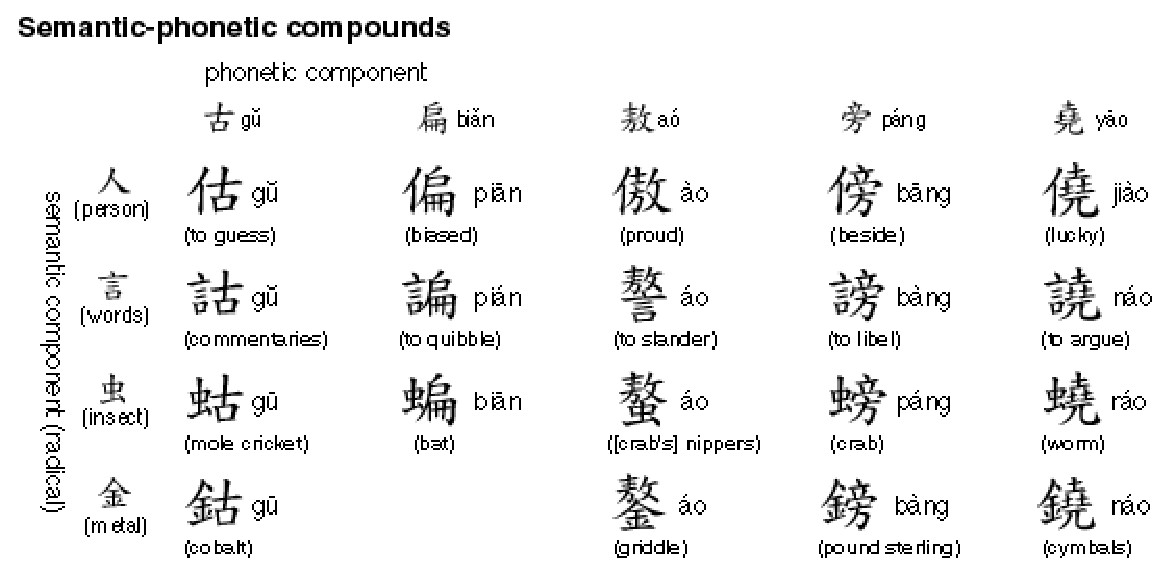
\includegraphics{../pics/hanzi-4.eps}

97\% of Chinese characters are phonetic compounds (Sproat 2010)!  Other estimates are lower (Wang, pc 2013)




\myslide{An example from Ancient Egyptian}

 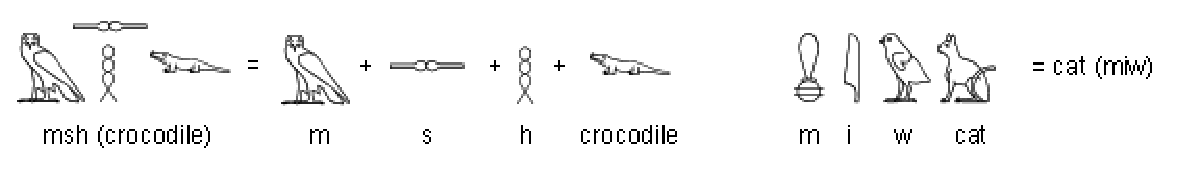
\includegraphics{../pics/hiero.eps}

Redundant, with both pronunciation and meaning!  Sometimes only one
would be used, sometimes the other, sometimes both.  Gradually
pronunciation won out and the characters were simplified and became
Hieratic and then Demotic.




\myslide{Relating writing systems to languages}

\begin{itemize}
\item There is never a simple correspondence between a writing system
  and a language.
\item For example, English uses the Roman alphabet, but Arabic numerals (e.g., 3 and 4 instead of III and IV).
\item Even when a new alphabet is designed, pronunciation changes.

\end{itemize}







% \myslide{Japanese}

% Japanese: logographic system kanji, syllabary katakana, syllabary hiragana kanji: 5,000-10,000 borrowed Chinese characters katakana
% used mainly for non-Chinese loan words, onomatopoeic words, foreign names, and for emphasis

% hiragana
% originally used only by women (10th century), but codified in 1946 with 48 syllables used mainly for word endings, kids’ books, and for words with obscure kanji symbols

% romaji: Roman characters


% \myslide{Korean}



% “Korean writing is an alphabet, a syllabary and logographs all at once.” (http://home.vicnet.net.au/∼ozideas/writkor.htm) The hangul system was developed in 1444 during King Sejong’s reign.
% There are 24 letters: 14 consonants and 10 vowels But the letters are grouped into syllables, i.e. the letters in a syllable are not written separately as in the English system, but together form a single character. E.g., “Hangeul” (from: http://www.omniglot.com/writing/korean.htm):




% Transcription Why speech is hard to represent Articulation Measuring sound

% In South Korea, hanja (logographic Chinese characters) are also used.

% Acoustics


% \myslide{Azeri}

% A Turkish language with speakers in Azerbaijan, northwest Iran, and (former Soviet) Georgia 7th century until 1920s: Arabic scripts. Three different Arabic scripts used 1929: Latin alphabet enforced by Soviets to reduce Islamic influence. 1939: Cyrillic alphabet enforced by Stalin 1991: Back to Latin alphabet, but slightly different than before. → Latin typewriters and computer fonts were in great demand in 1991









\myslide{Comparison of writing systems}



The pros and cons of each type of system depend on a variety of factors: 
\begin{itemize}
\item Accuracy:  Can every word be written down accurately?
\item Learnability: How long does it take to learn the system?
\item Cognitive ability: Are some systems unnatural? (e.g. Does dyslexia show that alphabets are unnatural?)
\item Language-particular differences: English has thousands of
  possible syllables; Japanese has very few in comparison (52, modulo
  vowel length)
\item Connection to history/culture: Is there meaning in the system
  beyond its use as a writing system?
  \newpage
\item Some languages have changed scripts (sometimes more than once):
  \begin{itemize}
  \item  Malay: pallava (Brahmic),  jawi (Arabic), alphabet
  \item  Korean: hanja (Chinese), hangul
  \item Mongolian: Hudum Mongol bichig (Old Uygar, from Aramaic), Cyrillic
  \end{itemize}
\item Many languages have had orthographic reforms
  \begin{itemize}
  \item American Spelling (English)
    \begin{itemize}
    \item \eng{authour} $\rightarrow$ \eng{author}
    \end{itemize}
  \item Japanese post-war reform (actually started pre-war)
    \begin{itemize}
    \item  蝶   てふ \jpn{tefu} $\rightarrow$  ちょう
      \jpn[chi-xyo-u]{chou} ``butterfly''
    \item  居る ゐる \jpn{wiru} $\rightarrow$  いる \jpn{iru} ``be''
  \end{itemize}

\item New Rumi Spelling/Ejaan Yang Disempurnakan (Malay/Indonesian) in 1972
  \begin{itemize}
  \item \zsm{di-buat} $\rightarrow$ 	\zsm{dibuat}, \zsm{di-rumah} $\rightarrow$ \zsm{di
    rumah}
  \item \zsm{ch/tj} \ipa{/tʃ/} $\rightarrow$ \zsm{c}: \zsm{tjicak/chicak}  $\rightarrow$
    \zsm{cicak}
  \item   \zsm{njonja/nyonya}	 $\rightarrow$ \zsm{nyonya}
  \end{itemize}
\end{itemize}
\end{itemize}








\myslide{Encoding written language}
\begin{itemize}
\item Information on a computer is stored in \textbf{bits}.
\item A bit is either on (= 1, yes) or off (= 0, no).
\item A list of 8 bits makes up a byte, e.g., 01001010
\item Just like with the base 10 numbers we're used to, the order of the bits in a byte matters:
  \begin{itemize}
  \item Big Endian: most important bit is leftmost (the standard way of doing things)
  \item Little Endian: most important bit is rightmost (only used on Intel machines)
  \end{itemize}
\end{itemize}

\myslide{How much information in a byte?}

\begin{itemize}
\item Every bit encodes two states (1 or 0)
\item $n$ bits encodes $2^n$ states
  \begin{itemize}
  \item $2 \times 2 \times 2 \times 2$ \ldots $n$ times
  \end{itemize}
\item So 8 bits encodes $2^8$ or 256 things
\end{itemize}







\myslide{An encoding standard: ASCII}

\begin{itemize}
\item  With 256 possible characters, we can store:
  \begin{itemize}
  \item every single letter used in English,
  \item plus all the things like commas, periods, space bar, percent sign (\%), back space, and so on.
  \end{itemize}
\item \textbf{ASCII} = the American Standard Code for Information Interchange
  \begin{itemize}
  \item  7-bit code for storing English text
  \item 7 bits = 128 possible characters.
  \item The numeric order reflects alphabetic ordering.
  \end{itemize}
\end{itemize}





\myslide{The ASCII chart}
Codes 1–31 are used for control characters (backspace, return, tab, \ldots).
\begin{center}
  
{\tt\small 
  \begin{tabular}{cccccccccccc}
    032 & \textvisiblespace &048 & 0 &064& @ &080 & P &096& `   &112& p \\      
    033 & !                 &049 & 1 &065& A &081 & Q &097& a   &113& q \\    
    034 & "                 &050 & 2 &066& B &082 & R &098& b   &114& r \\    
    035 & \#                &051 & 3 &067& C &083 & S &099& c   &115& s \\    
    036 & \$                &052 & 4 &068& D &084 & T &100& d   &116& t \\    
    037 & \%                &053 & 5 &069& E &085 & U &101& e   &117& u \\    
    038 & \&                &054 & 6 &070& F &086 & V &102& f   &118& v \\    
    039 & `                 &055 & 7 &071& G &087 & W &103& g   &119& w \\    
    040 & (                 &056 & 8 &072& H &088 & X &104& h   &120& x \\    
    041 & )                 &057 & 9 &073& I &089 & Y &105& i   &121& y \\    
    042 & *                 &058 & : &074& J &090 & Z &106& j   &122& z \\    
    043 & +                 &059 & ; &075& K &091 & [ &107& k   &123& \{ \\   
    044 & '                 &060 & < &076& L &092 & $\backslash$ & 108 &l &124& \_ \\ 
    045 & -                 &061 & = &077& M &093 & ]  &109& m   &125& \} \\   
    046 & .                 &062 & > &078& N &094 & $\wedge$ &110& n &126& $\sim$\\   
    047 & /                 &063 & ? &079& O &095 & \char`\_& 109 &o&127& DEL \\ 
  \end{tabular}
}
\end{center}    
    
\myslide{What if 127 characters isn't enough?}

\begin{itemize}
\item Local Variants
  \begin{itemize}
  \item[{[092]}] Japanese ASCII: Yen ({\ooalign{Y\crcr$=$}}) instead of backslash
    ($\backslash$)
  \item[{[035]}] UK ASCII: Pounds Sterling ($\textsterling$) instead of hash (\#).
  \end{itemize}
\item But what if you need more letters?
  \begin{itemize}
  \item Transliteration
    % \item Composition
  \item Multi-byte encodings
  \end{itemize}
\end{itemize}


% \myslide{E-mail issues}
% Mail sent on the internet used to only be able to transfer the 7-bit ASCII messages. But now we can detect the incoming character set and adjust the input. Note that this is an example of meta-information = information which is printed as part of the regular message, but tells us something about that message. Multipurpose Internet Mail Extensions (MIME) provides meta-information on the text, which tells us:
% which version of MIME is being used what the charcter set is if that character set was altered, how it was altered
% Mime-Version: 1.0 Content-Type: text/plain; 7bit


% charset=US-ASCII Content-Transfer-Encoding:



\myslide{Transliteration}

\begin{itemize}
\item Use ASCII, and fake the missing letters
  \begin{itemize}
  \item ue for \"u, oe for \"o, \ldots
  \end{itemize}
\item \blu{Volapuk} replaces Cyrillic letters with Latin ones in order to look the same as typed or handwritten Cyrillic letters.
  \begin{enumerate}
  \item Replace ``the same'' letters: a, e, K, M, T, o, y.
  \item    Replace similar-looking letters: $\Gamma$  with 2 (handwritten resemblance) or r,\ldots
  \item Replace all other non-obvious hard-to-represent characters;
    there are many options for each letter: $\Phi$ with qp or 0. The choice for each letter
    depends on the preferences of the individual user.
  \end{enumerate}
\item These transliterations are hard to read, but better than nothing
\end{itemize}


\myslide{Different coding systems}

\begin{itemize}
\item Extended ASCII (use 256 characters)
\item Other encodings
  \begin{itemize}
  \item ISO 8859-1: includes extra letters for French, German, Spanish, \ldots
  \item ISO 8859-5: Cyrillic alphabet
  \item ISO 8859-7: Greek alphabet
  \item ISO 8859-8: Hebrew alphabet 
  \end{itemize}
\item But you can only have one encoding at a time!
  \begin{itemize}
  \item  You can't have both Greek and Russian
  \end{itemize}
\item 256 characters is not enough for many languages
\end{itemize}


\myslide{Multi-byte Encodings}

\begin{itemize}
\item Use more bytes
\item EUC-JP (Extended Unix Code Japanese)
  \begin{itemize}
  \item An ASCII character is represented by one byte, with the first bit 0.
  \item A character from JIS-X-0208 (code set 1) is represented by two
    bytes, both with the first bit 1.
    \begin{itemize}
    \item  This includes Hiragana, Katakana and most Chinese Characters.
    \end{itemize}
  \item A character from JIS-X-0212 (code set 3) is represented by
    three bytes, the first being 0x8F, and the second two both with the first bit 1.
    \begin{itemize}
    \item  This includes many more Chinese characters.
    \end{itemize}
  \end{itemize}
 This encoding scheme allows the easy mixing of 7-bit ASCII and 8-bit Japanese.
\end{itemize}

\myslide{Example of EUC-JP}


\begin{tabular}{cccccccccc}
  犬 & は & d & o & g & だ & 。& EOF \\
 b8a4 & a4cf & 64 & 6f & 67 & a4c0 &a1a3 &0a\\
\end{tabular}

\begin{itemize}
\item Written in hexadecimal: 0123456789ABCDEF  
  \begin{itemize}
  \item 0 = 0000 = 0  (0 + 0 + 0 + 0)
  \item 1 = 0001 = 1  (0 + 0 + 0 + 1)
  \item 2 = 0010 = 2  (0 + 0 + 2 + 0)
  \item 4 = 0100 = 4  (0 + 4 + 0 + 0)
  \item 8 = 1000 = 8  (8 + 0 + 0 + 0)
    \item[\ldots]
  \item A = 1010 = 10 (8 + 0 + 2 + 0)
    \item[\ldots]
  \item E = 1110 = 14 (8 + 4 + 2 + 0)
  \item F = 1111 = 15 (8 + 4 + 2 + 1)
  \end{itemize}
\item Bit one = 1 $\Rightarrow$ $> 8$
\item So  \texttt{b8a4} is \texttt{1011\,1000 1010\,0100}

\end{itemize}

\myslide{Problems with stateless encodings}

\begin{itemize}
%\CJKfamily{min}
\item Shift-JIS takes a different approach
\item each character is two bytes, so you can use the 8th bit
\item the trouble is you have to know where you are, \ldots
  \begin{itemize}
  \item Consider the following:
    \fbox{\begin{tabular}[t]{cccll}
      剣 & 道 & & \jpn[kendo]{kendo} \\
      \blu{8C95} & 93B9 \\
      白 & 血 & 病 \\
      9492 & 8C\blu{8C} & \blu{95}61 & \jpn[leukemia]{hakketsubyō}\\
    \end{tabular}}
  \item  剣 \blu{8C95} matches across character boundaries
    \begin{itemize}
    \item but you don't want to match it here
    \end{itemize}
  \end{itemize}
  \item When you delete a character, you need to know how many bytes it is
\end{itemize}
%\CJKfamily{gbsn}
\myslide{Still more problems}

\begin{itemize}
\item EUC-JP is stateful so it can't fit all characters
  \begin{itemize}
  \item using one bit to show state, so only: $2^{14}$ = 16,384
  \end{itemize}
\item You need to know what the encoding is:
\begin{itemize}
\item "文字化ã[]‘" (文字化け)
\end{itemize}
\end{itemize}

\noindent Much more in: \\
\bibentry{Lunde:1999}

\myslide{Unicode}

\begin{itemize}
\item Unicode solves many of these problems
  \begin{quote}
    “Unicode provides a unique number for every character, no matter what the platform, no matter what the program, no matter what the language.” (\url{www.unicode.org})
\end{quote}
\end{itemize}


\myslide{How big is Unicode?}


\begin{itemize}
\item Version 3.2 (2002) has codes for 95,221 characters from alphabets, syllabaries and logographic systems.
\item Uses 32 bits (4 bytes) 
  \\ Can represent $2^{32}$ = 4, 294, 967, 296 characters.
\item 4 billion possibilities for each character?
\item That takes a lot of space on the computer!
  \begin{itemize}
  \item Four times as much as ASCII
  \end{itemize}
\item Unicode 11.0 (2018) contains 137,439 characters
  covering 146 modern and historic scripts, as well as multiple symbol
  sets and emoji.
\item Version 15.1 (2023)  defines 149,813 character covering 161 scripts 
\end{itemize}

\myslide{Compact encoding of Unicode characters}

\begin{itemize}
\item UTF-32 (32 bits): direct representation
\item UTF-16 (16 bits): $2^{16}$ = 65,536 (subset!)
\item UTF-8 (variable width encoding)\\[2ex]
{\small
  \hspace*{-3em}\begin{tabular}{llllll}
  U+0000-U+007F 	&0xxxxxxx &         &         &          & ASCII\\
  U+0080-U+07FF 	&110yyyxx &10xxxxxx &         &          & Alphabets/Syllabaries\\
  U+0800-U+FFFF 	&1110yyyy &10yyyyxx &10xxxxxx &          & Logographs  \\
  U+10000-U+10FFFF      &11110zzz &10zzyyyy &10yyyyxx &10xxxxxx  & Room to expand

\end{tabular}}
\item First byte says how many will follow
\end{itemize}  

Nice consequence: ASCII text is in a valid UTF-8 encoding.



\myslide{How do we type everything in?}


\begin{itemize}
\item Use a keyboard tailored to your specific language
\item e.g. Highly noticeable how much slower your English typing is when using a Danish-designed keyboard.
\item Use a processor that allows you to switch between different character systems.
  \begin{itemize}
  \item e.g. Type in Cyrillic characters on your English keyboard.
  \end{itemize}
\item Use combinations of characters.
  \begin{itemize}
  \item e.g. An e followed by an {'} might result in an \'e.
  \end{itemize}
\item Pick and choose from a table of characters.
\end{itemize}






\myslide{Unwritten languages}




Many languages have never been written down. Of the 6,900 spoken
languages, approximately 3,000 have never been written down.

Some examples:
\begin{itemize}
\item Salar, a Turkic language in China.
\item Gugu Badhun, a language in Australia.
\item Southeastern Pomo, a language in California
\end{itemize}

Ongoing work in adding alphabets, often by Bible translators and linguists!



\myslide{Redundancy of Representation}

\begin{itemize}
\item You can remove a lot of information and still understand
  \begin{itemize}
  \item For example, with no vowels, spaces or segmentation
  \item  F C T S R S T R N G R T H N F C T N
    \\ \hide{Facts are stranger than fiction}
  \end{itemize}
\item It is much easier if you know the meaning
\item Redundancy is important if there is \emp{noise}
\item There is normally a lot of noise, so all natural languages are redundant
\end{itemize}

% \myslide{Another Example}

% \begin{quote}
% Before the \wt{addition} of the \wt{parity} check-bits in
% \wt{Hamming's} code we \wt{were} - intuitively - dealing \wt{with}
% pure information. \wt{The} extra symbols \wt{added} did not
% \wt{change} the amount \wt{of} information that \wt{was} being
% conveyed \wt{and} so we \wt{say} that this \wt{was} redundant.
% \end{quote}

% \begin{itemize}
% \item Redundancy is useful
% \end{itemize}

\myslide{Efficient Representation}

\begin{itemize}
\item Language is also efficient in its coding
\item Consider the most common 20 words of English:
\\ \textit{the, of, and, a, to, in, is, you, that, it, he, was, for, on, are, as, with, his, they, I}
\item They are all short!
\item Frequent expressions are shortened
\\ \textit{today} not \textit{on this day}
\item This makes the overall text shorter
\end{itemize}


\myslide{Playing with Writing: Acrostics}
\begin{flushleft}\small
  To the Members of the California State Assembly:\\ I am returning
  Assembly Bill 1176 without my signature.

  For some time now I have lamented the fact that major issues are overlooked while many \\
  unnecessary bills come to me for consideration. Water reform, prison
  reform, and health \\
  care are major issues my Administration has brought to the table, but the
  Legislature just \\
  kicks the can down the alley.

  Yet another legislative year has come and gone without the major
  reforms Californians  \\ overwhelmingly deserve. In light of this, and
  after careful consideration, I believe it is \\ unnecessary to sign
  this measure at this time.

  Sincerely, Arnold Schwarzenegger
\end{flushleft}
{\small
Wired (2009) ``SCHWARZENEGGER FLIPS OFF LAWMAKERS IN HIDDEN MESSAGE''
\url{https://www.wired.com/2009/10/schwarzenegger/}
}
\myslide{Playing with Writing: Acrostics}
\begin{flushleft}\small
  To the Members of the California State Assembly:\\
 \blu{I} am returning   Assembly Bill 1176 without my signature. 

\blu{F}or some time now I have lamented the fact that major issues are overlooked while many \\
\blu{u}nnecessary bills come to me for consideration. Water reform, prison reform, and health \\
\blu{c}are are  major issues my Administration has brought to the table, but the Legislature just \\
\blu{k}icks the can down the alley.

\blu{Y}et another legislative year has come and gone without the major reforms Californians \\
\blu{o}verwhelmingly deserve. In light of this, and after careful consideration, I believe it is \\
\blu{u}nnecessary to sign this measure at this time.

  Sincerely, Arnold Schwarzenegger
\end{flushleft}


\myslide{Playing with Writing: Hanzi}

\begin{itemize}
\item {\Large 目田 氏王} \textit{mùtián sh\={\i}wáng} ``eye-field clan-king''
\end{itemize}

\myslide{Playing with Writing: Graphemic Puns}

\begin{itemize}
\item {\Large 目田 氏王} \textit{mùtián sh\={\i}wáng} ``eye-field clan-king''
\item {\Large 自由 民主} \textit{zìyóu m\'{\i}nzh\v{u}} ``freedom democracy'' 
  \begin{itemize}
  \item Just like freedom and democracy but missing a bit
  \item Not caught by censors (at first)
  \end{itemize}
\end{itemize}

{\small 
Victor Mair (2010) ``Decapitated Democracy, Headless Liberty''\\ \textit{Language Log} 
\url{http://languagelog.ldc.upenn.edu/nll/?p=2614}}

% \myslide{Representing Speech}


% \myslide{The need for speech}

% \begin{itemize}
% \item We want to be able to encode any spoken language
%   \begin{itemize}
%   \item What if we want to work with an unwritten language?
%   \item What if we want to examine the way someone talks and don’t have time to write it down?
%   \end{itemize}
% \item Many applications for encoding speech:
%   \begin{itemize}
%   \item Building spoken dialogue systems, i.e. speak with a computer (and have it speak back).
%   \item Helping people sound like native speakers of a foreign language.
%   \item Helping speech pathologists diagnose problems
%   \end{itemize}
% \end{itemize}






% \myslide{What does speech look like?}




% We can transcribe (write down) the speech into a phonetic alphabet. 
% \begin{itemize}
% \item It is very expensive and time-consuming to have humans do all the transcription.
% \item To automatically transcribe, we need to know how to relate the
%   audio signal to the individual sounds that we hear.
% \item  We need to know:
% \begin{itemize}
% \item some properties of speech
% \item how to measure these speech properties
% \item how these measurements correspond to sounds we hear
% \end{itemize}
% \end{itemize}







% \myslide{What makes representing speech hard?}
% \begin{itemize}
% \item Sounds run together, and it’s hard to tell where one sound ends and another begins.
% \item People say things differently from one another: 
%   \begin{itemize}
%   \item People have different dialects
%   \item People have different size vocal tracts 
%   \end{itemize}
% \item Hand written text shares similar problems
% \newpage
% \item People say things differently across time: What we think of as one sound is not always (usually) said the same
% \item coarticulation = sounds affecting the way neighboring sounds are said
% \\e.g. k is said differently depending on if it is followed by ee or by oo.

% \item What we think of as two sounds are not always all that different.
% \\ e.g. The \textit{s} in \textit{see} is acoustically very similar to the \textit{sh} in \textit{shoe}
% \end{itemize}




% \myslide{Articulatory properties: How it's produced}


% \begin{itemize}
% \item We could talk about how sounds are produced in the vocal tract, i.e. articulatory phonetics
% \begin{itemize}
% \item place of articulation (where): [t] vs. [k]
% \item manner of articulation (how): [t] vs. [s]
% \item voicing (vocal cord vibration): [t] vs. [d]
% \end{itemize}
% \item But unless the computer is modeling a vocal tract, we need to know acoustic properties of speech which we can quantify.
% \end{itemize}





% % \myslide{Measuring sound}

% % \begin{itemize}
% % \item Sound is actually a continuous wave
% % \item We store data at each discrete point, in order to capture the general pattern of the sound
% % \item sampling rate = how many times in a given second we extract a moment of sound; measured in samples per second Sound is continuous, but we have to store data in a discrete manner.
% % \end{itemize}

% % \myslide{Signal sampling representation.}
% % 
\includegraphics[height=\textheight]{../pics/sampling.eps} (wikipedia)



% % \myslide{Sampling rate}


% % The higher the sampling rate, the better quality the recording ... but the more space it takes. 

% % \begin{itemize}
% % \item Speech needs at least 8000 samples/second, but most likely 16,000 or 22,050 Hz will be used nowadays.
% % \item The rate for CDs is 44,100 samples/second (or Hertz (Hz))
% % \end{itemize}
% % Now, we can talk about what we need to measure









% % \myslide{Acoustic properties: What it sounds like}
% % \begin{itemize}
% % \item \blu{Sound waves} = “small variations in air pressure that occur very rapidly one after another”
% % \item The main properties we measure:
% %   \begin{itemize}
% %   \item speech flow = rate of speaking, number and length of pauses (seconds)
% %   \item loudness (amplitude) = amount of energy (decibels)
% %   \item frequency = how fast the sound waves are repeating (cycles per second, i.e. Hertz)
% %     \begin{itemize}
% %     \item pitch = how high or low a sound is
% %     \item In speech, there is a fundamental frequency, or pitch, along with higher-frequency overtones.
% %     \end{itemize}
% %   \end{itemize}
% % \end{itemize}

% % Researchers also look at things like intonation, i.e., the rise and fall in pitch



% % % \myslide{Speech Sample}
% % % \noindent\includegraphics[width=\textwidth]{../pics/BushAPlan.eps}


% % % Pitch track, transcription, spectogram and audio waveform.



% % \myslide{Measurement-sound correspondence}


% % \begin{itemize}
% % \item  How dark is the picture? $\rightarrow$ How loud is the sound?
% %   \begin{itemize}
% %   \item We measure this in decibels.
% %   \end{itemize}
% % \item Where are the lines the darkest? $\rightarrow$  Which frequencies are the loudest and most important?
% %   \begin{itemize}
% %   \item We can measure this in terms of Hertz, and it tells us what the vowels are.
% %   \end{itemize}

% % \item Speech signals are very different from text.
% %   \begin{itemize}
% %   \item No words!
% %   \end{itemize}
% % \end{itemize}

% \myslide{Relating Speech to Text}

% \begin{itemize}
% \item Speech can have
%   \begin{itemize}
%   \item loudness
%   \item intonation
%   \end{itemize}
% \item Text can have
%   \begin{itemize}
%   \item Different fonts, styles and size
%   \item Colour
%   \item Position
%   \item Explicit markup
%   \end{itemize}
% \item Both combine with other modes
%   \begin{itemize}
%   \item gestures
%   \item pictures
%   \end{itemize}
% \end{itemize}





% \myslide{Applications of speech encoding}


% \begin{itemize}
% \item Mapping sounds to symbols (alphabet), and vice versa, has some very practical uses.
%   \begin{itemize}
%   \item Automatic Speech Recognition (ASR): sounds to text
%   \item Text-to-Speech Synthesis (TTS): texts to sounds
%   \end{itemize}
% \item These are not easy tasks.
% \item Text-to-Speech Synthesis is somewhat easier.
% \end{itemize}



% \myslide{Automatic Speech Recognition (ASR)}

% \begin{itemize}
% \item Automatic speech recognition = process by which the computer maps a speech signal to text.
% \item Uses/Applications:
%   \begin{itemize}
%   \item Dictation
%   \item Dialogue systems
%   \item Telephone conversations
%   \item People with disabilities – e.g. a person hard of hearing could use an ASR system to get the text (closed captioning)
%   \item Spying (many agencies run ASR on phone conversations and search for keywords)
%   \item Indexing audio data
%   \end{itemize}
% \end{itemize}








% \myslide{Steps in an ASR system}

% \begin{enumerate}
% \item Digital sampling of speech
% \item Acoustic signal processing = converting the speech samples into particular measurable units
% \item Recognition of sounds, groups of sounds, and words 
% \end{enumerate}

% May or may not use more sophisticated analysis of the utterance to
% help. e.g., a [t] might sound like a [d], and so word information
% might be needed (more on this later)









% \myslide{Kinds of ASR systems}


% Different kinds of systems, with an accuracy-robustness tradeoff: 

% \begin{itemize}
% \item Speaker dependent = work for a single speaker
% \item Speaker independent = work for any speaker of a given variety of a language, e.g. American English
% \item A common type of system starts general, but learns: 
% \begin{itemize}
% \item Speaker adaptive = start as independent but begin to adapt to a single speaker to improve accuracy
% \item Adaptation may simply be identifying what type of speaker a person is and then using a model for that type of speaker
% \end{itemize}
% \end{itemize}








% \myslide{Kinds of ASR systems}

% \begin{itemize}
% \item Differing sizes and types of vocabularies
% \begin{itemize}
% \item from tens of words to tens of thousands of words
% \item normally very domain-specific, e.g., flight vocabulary
% \end{itemize}
% \item continuous speech vs. isolated-word systems:
% \begin{itemize}
% \item \blu{continuous speech systems} = words connected together and not separated by pauses
% \item \blu{isolated-word systems} = single words recognized at a time, requiring pauses to be inserted between words 
%   \begin{itemize}
%   \item easier to find the endpoints of words
%   \item harder to use
%   \end{itemize}
% \end{itemize}
% \end{itemize}


% \myslide{How good are the systems?}

% \begin{itemize}
% \item Dictation: 1-2\% Word Error Rate
%   \begin{itemize}
%   \item speakers who match the training data
%   \item after system adaptation
%   \item a clean noise environment (e.g. quiet office or laboratory space).
%   \end{itemize}
% \item Noisy room, multiple speakers 50+\% WER
% \end{itemize}




% \myslide{Text-to-Speech Synthesis (TTS)}
% \begin{itemize}
% \item Could just record a voice saying phrases or words and then play back those words in the appropriate order.
% \item This won’t work for, e.g., dialogue systems where speech is generated on the fly.
% \item Or can break the text down into smaller units
%   \begin{enumerate}
%   \item Convert input text into phonetic alphabet (\emp{ambiguous} mapping)
%   \item Synthesize phonetic characters into speech 
%   \end{enumerate}
% \item  To synthesize characters into speech, people have tried:
%   \begin{itemize}
%   \item using a model based on frequencies, the loudness, etc.
%   \item using a model of the vocal tract and human speech production
%   \end{itemize}
% \end{itemize}



% \myslide{Synthesizing Speech}

% \begin{itemize}
% \item In some sense, TTS really is the reverse process of ASR
%   \begin{itemize}
%   \item Since we know what frequencies correspond to which vowels, we can play those frequencies to make it sound like the right vowel.
%   \item However, sounds are always different (across time, across speakers)
%   \end{itemize}
% \item One way to generate speech is to have a database of speech and to use the diphones, i.e., two-sound segments, to generate sounds.
% \item Diphones help with the context-dependence of sounds
% \end{itemize}






% \myslide{It’s hard to be natural}
% When trying to make synthesized speech sound natural, we encounter the same problems as what makes speech encoding hard: 

% \begin{itemize}
% \item The same sound is said differently in different contexts.
% \item Different sounds are sometimes said nearly the same.
% \item Different sentences have different intonation patterns. 
% \item Lengths of words vary depending on where in the sentence they are spoken. 
%     \begin{enumerate}
%     \item The \blu{car} crashed into the tree.
%     \item It’s my \blu{car}.
%     \item \blu{Cars}, trucks, and bikes are vehicles.
%     \end{enumerate}
%   \end{itemize}









% \myslide{Speech to Text to Speech}



% If we convert speech to text and then back to speech, it should sound the same.
% \begin{itemize}
% \item  But at the conversion stages, there is information loss.
% \item To avoid this loss would require a lot of memory and knowledge about what exact information to store.
% \item The process is thus irreversible.
% \item In fact, people can't say the same sentence exactly the same way either!
% \end{itemize}

\myslide{Speech vs Writing (1): Time-bound}

\begin{itemize}
\item \subhead{Speech}

\begin{itemize}
\item time-bound
\item dynamic, transient
\item normally direct between a speaker and a known addressee
\end{itemize}
\item \subhead{Writing}
\begin{itemize}
\item space-bound
\item static, permanent
\item normally indirect with the addressee unknown
\end{itemize}
\end{itemize}
Summary of Table~2.1 (pp 28--30) in \bibentry{Crystal:2006}. (\blu{conversation vs books})


\myslide{Speech vs Writing (2): Spontaneous}

\begin{itemize}
\item \subhead{Speech}

\begin{itemize}
\item no lag between production and reception
\item hard to plan complex constructions
\item[$\Rightarrow$] repetitions, rephrasing, comments clauses
\item Sentence boundaries often unclear
\end{itemize}
\item \subhead{Writing}
\begin{itemize}
\item lag between production and reception
\item readers can reread and analyse in depth
\item[$\Rightarrow$] careful organization and compact expressions
\item Sentence (and paragraph, \ldots) boundaries are clear \com{English!}
\end{itemize}
\end{itemize}


\myslide{Speech vs Writing (3): Face-to-Face}

\begin{itemize}
\item \subhead{Speech}

\begin{itemize}
\item Extralinguistic cues are common (facial expressions, gestures)
\item Immediate feedback (back channel)
\item Deictic expressions are common (referring to the situation)
\\ \eng{that one, you, now, over there}
\end{itemize}
\item \subhead{Writing}
\begin{itemize}
\item Different extralinguistic possibilities (fonts, color, pictures)
\item No immediate feedback
\item Fewer deictic expressions
\end{itemize}
\end{itemize}


\myslide{Speech vs Writing (4): Loosely Structured}

\begin{itemize}
\item \subhead{Speech}

\begin{itemize}
\item Contractions are common: \eng{isn't, he's}
\item Long coordinate sentences are common
\item informal vocabulary: \eng{thingamajig, whatsit}
\item obscenity more common
\end{itemize}
\item \subhead{Writing}
\begin{itemize}
\item Subordination more common (relative clauses)
\item Longer sentences (can be multipage)
\item Some items rarely pronounced: \(  H(\mathrm{p}) = -\sum_{x \in X} \mathrm{p}(x)\log_2\mathrm{p}(x) \)
\end{itemize}
\end{itemize}


\myslide{Speech vs Writing (5): Socially Interactive}

\begin{itemize}
\item \subhead{Speech}

\begin{itemize}
\item Well suited to social functions
  \begin{itemize}
  \item greetings
  \item maintaining social relationships
  \item expression attitudes and opinions
  \end{itemize}
Much use of prosody and non-verbal features
\end{itemize}
\item \subhead{Writing}
\begin{itemize}
\item Suited to recording facts and communicating ideas
\item Easier to scan
\item Tables demonstrate relations between things
\item Text can be read at one's own pace
\end{itemize}
\end{itemize}


\myslide{Speech vs Writing (6): Immediately Revisable}

\begin{itemize}
\item \subhead{Speech}

\begin{itemize}
\item You can rephrase at once, based on feedback
\item Errors once spoken can't be withdrawn
\item Interruptions and overlap is common
\end{itemize}
\item \subhead{Writing}
\begin{itemize}
\item You can remove errors without the speaker ever seeing them
\item Once published errors can only be withdrawn through revisions
\item Interruptions are not visible
\end{itemize}
\end{itemize}


\myslide{Speech vs Writing (7): Prosodically Rich}

\begin{itemize}
\item \subhead{Speech}

\begin{itemize}
\item Prosody
\\ intonation; loudness; tempo; rhythm, pause tone of voice
\end{itemize}
\item \subhead{Writing}
\begin{itemize}
\item Pages, lines, capitalization, spatial organization
\item Punctuation (?!.)
\item \textbf{Fonts}, \textsc{capitalization}, \textit{style} 
\item Tables, graphs, formulae
\end{itemize}
\end{itemize}

% \myslide{Speech vs Writing (X)}

% \begin{itemize}
% \item \subhead{Speech}

% \begin{itemize}
% \item 
% \end{itemize}
% \item \subhead{Writing}
% \begin{itemize}
% \item 
% \end{itemize}
% \end{itemize}


% \myslide{Online Demos}

% \begin{itemize}
% \item AT\&T mulitilingual TTS system: http://www.research.att.com/projects/tts/demo.php
% \item various systems and languages: http://www.ims.uni-stuttgart.de/∼moehler/synthspeech/
% \item Nuance Realspeak: http://www.nuance.com/realspeak/demo/default.asp
% \end{itemize}






% \myslide{Language Modeling}




% \myslide{N-grams: Motivation}

% Let’s say we’re having trouble telling what word a person said in an ASR system
% \begin{itemize}
% \item We could look it up in a phonetic dictionary
% \item But if we hear something like ni, how can we tell if it’s \textit{knee, neat, need,} or some other word?
% \item All of these are plausible words
% \newpage
% \item We can assign a probability, or weight, to each change:
%   \begin{itemize}
%   \item deleting a [t] at the end of a word is slightly more common than deleting a [d]
%   \item We can look at how far off a word is from the pronunciation;
%   \item We’ll return to the issue of minimum edit distance with spell checking
%   \end{itemize}

% \item But if the previous word was \textit{I}, the right choice becomes clearer ...
%   \begin{itemize}
%   \item \textit{I knee} 
%   \item \textit{I neat}
%   \item \textit{I need}
%   \end{itemize}
% \end{itemize}
% (Material based upon chapter 5 of Jurafsky and Martin 2000)






% \myslide{Back to N-grams}


% \begin{itemize}
% \item An n-gram is a stretch of text $n$ words long
% \item Approximation of language: information in n-grams tells us something about language, but doesn’t capture the structure
% \item Efficient: finding and using every, e.g., two-word collocation in a text is quick and easy to do
% \item N-grams help a variety of NLP applications, including word prediction
% \begin{itemize}
% \item We can predict the next word of an utterance, based on the previous 
%   $n - 1$ words
% \end{itemize}
% \end{itemize}







% \myslide{Simple n-grams}



% How to predict the next word, based on the previous context

% \begin{itemize}
% \item Consider \textit{I dreamed I saw the knights in}
% \item Find is the likelihood of $w_7$ being the next word, given that we've seen $w_1, \ldots, w_6$
% \item So, we’ll have to examine $P(w_1, \ldots, w_6)$
%   \begin{itemize}
%   \item $= P(w_1)P(w_2|w_1)P(w_3|w_2,w_1)\ldots$
%   \end{itemize}

% \item  For large $n$ the probabilities are impractical to calculate:
%   \begin{itemize}
%   \item They occur sparsely
%   \item There are too many to store
%   \end{itemize}
%   \end{itemize}







% \myslide{How big should $n$ be?}

% \begin{itemize}
% \item Approximate with lower $n$
%   \begin{itemize}
%   \item For speech-to-text 3 (words) seems to be the best
%   \item For text-to-speech 2 (phonemes) seems to be the best
%   \item For machine translation 7 seems to be the best (so far)
%   \end{itemize}
% \item But there are some structures $n$ grams just don't get
%   \begin{itemize}
%   \item \textit{The \blu{book} that yesterday I thought of maybe \blu{buying} for a friend}
%   \item  \glll \blu{けして} その よう な こと {で は あり} \blu{ません} \\
%     keshite sono you na koto de-ha-ari masen \\
%     definitely that kind of thing is not \\
%     (\blu{keshite} can only be used in negative contexts)
%   \item We call these \blu{long distance dependencies}
   
%   \end{itemize}
% \end{itemize}



% \myslide{Bigrams}


% Alphabetic Syllabic

% bigrams (n = 2) are a better choice and still easy to calculate: (7) P (wn |w1 , ..., wn−1 ) ≈ P (wn |wn−1 ) (8) P (over |The , quick , brown, fox , jumped ) ≈ P (over |jumped ) And thus, we obtain for the probability of a sentence: (9) P (w1 , ..., wn ) = P (w1 )P (w2 |w1 )P (w3 |w2 )...P (wn |wn−1 )

% Logographic 







% \myslide{Bigram example}


% What is the probability of seeing the sentence The quick brown fox jumped over the lazy dog? (10) P(The quick brown fox jumped over the lazy dog) = P (The |START)P (quick |The )P (brown|quick )...P (dog |lazy ) Or, for our ASR example, we can compare: (11) P (need |I) >> P (neat |I)


\myslide{Comparison of speed for different modalities}
% http://en.wikipedia.org/wiki/Words_per_minute

Speed in words per minute (one word is 6 characters)
\\ (English, computer science students, various studies)

\begin{tabular}{lrl}
 Activity           & Speed (wpm) & Comments \\ \hline
  Reading            & 300 & 200 (proof reading)\\
  Writing              & 31 & 21 (composing) \\ 
  Speaking             & 150 & \\
  Hearing              & 150 & 210 (speeded up)  \\
  Typing               & 33  & 19 (composing) 
\end{tabular}
\begin{itemize}
\item Reading $>>$ Speaking/Hearing $>>$ Typing
  \begin{itemize}
  \item[$\Rightarrow$] Speech for input
  \item[$\Rightarrow$] Text for output
  \end{itemize}
\end{itemize}

Does anyone know of work on languages other than English?


\myslide{Summary}

\begin{itemize}
\item There are many ways to represent text
\item Some are easier to encode than others
\item Efficient representation is not always the goal
\item Speech can be very different from text
%\item It is non-trivial to convert between them
\end{itemize}


% \myslide{Further Readings}

% \myslide{Unsolicited Advice}

% \begin{itemize}
% \item Following instructions carefully is a really useful skill
% \item \textit{Measure twice cut once}
% \item Always proofread something before you expose it to others
% \end{itemize}

\myslide{Acknowledgments}

\begin{itemize}
\item Many slides taken from Marcus Dickinson
\item Much of the information on writing systems and the graphics used are taken from the great site \url{http://www.omniglot.com}
\end{itemize}

\myslide{Just for interest}


\myslide{A writing system  with an unusual realization: Braille}
\begin{itemize}
\item Tactile
  \begin{itemize}
  \item Braille is a writing system that makes it possible to read and write through touch; primarily used by the (partially) blind.
  \item It uses patterns of raised dots arranged in cells of up to six dots in a $3 \times 2$ configuration.
    \begin{itemize}
    \item How many bits is this? % 6
    \item How many characters can be represented? % (* 2 2 2 2 2 2) 64
    \end{itemize}
  \item Each pattern represents a character, but some frequent words and letter combinations have their own pattern.
  \end{itemize}
\end{itemize}

\myslide{Braille alphabet}

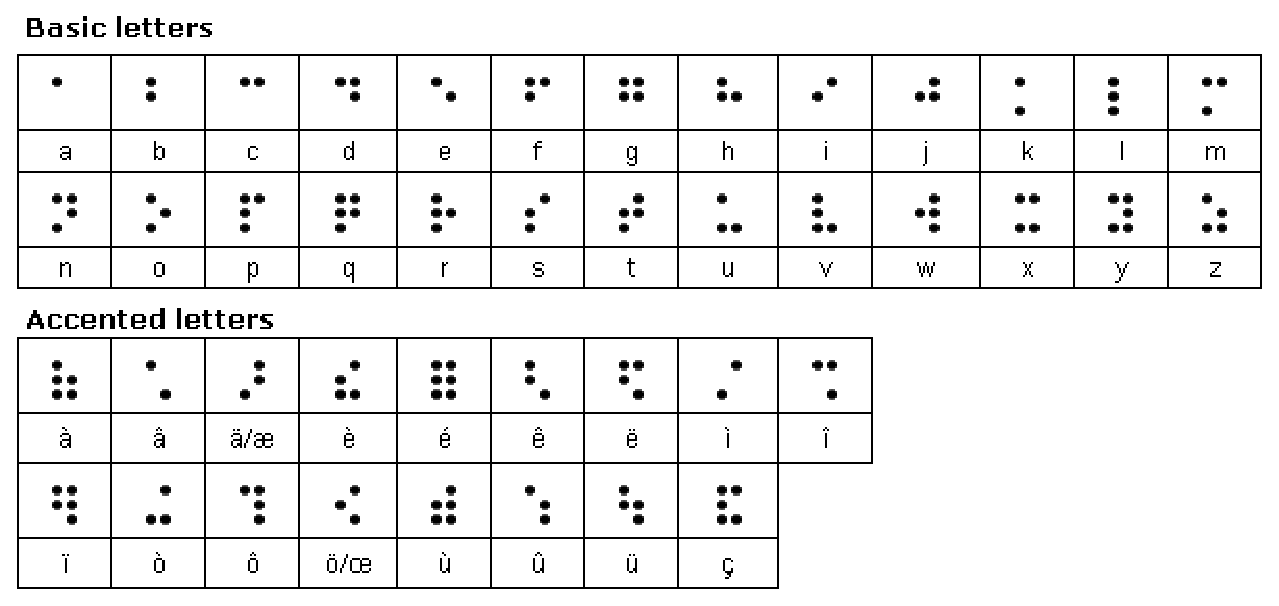
\includegraphics{../pics/braille_basic.eps}
\newpage
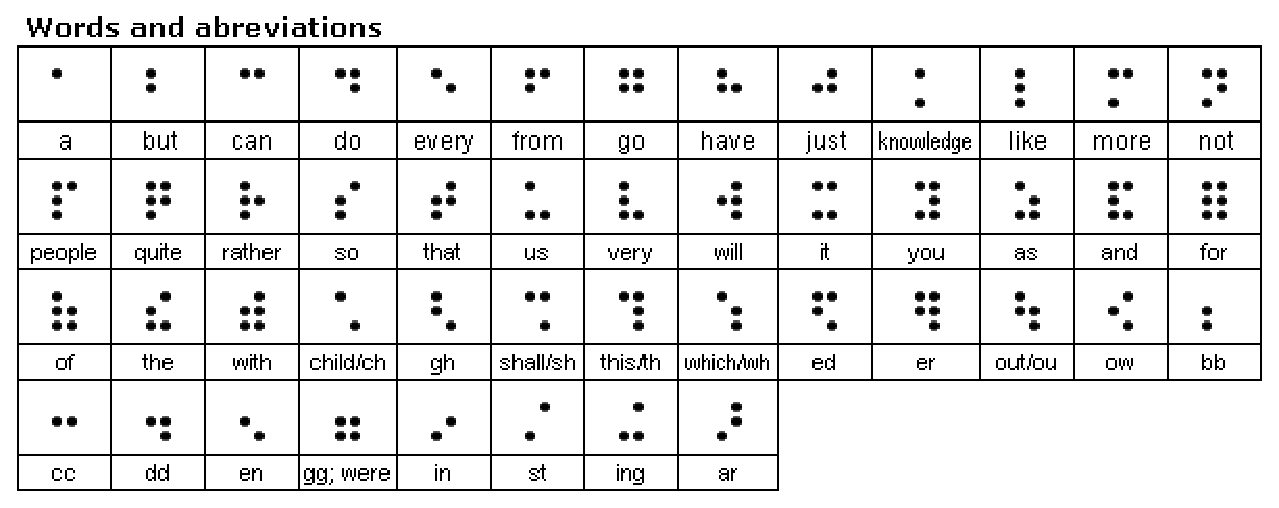
\includegraphics{../pics/braille_abbrr.eps}

Braille terminals (refreshable Braille displays) push the pins up in
real time

\myslide{Braille Secrets}

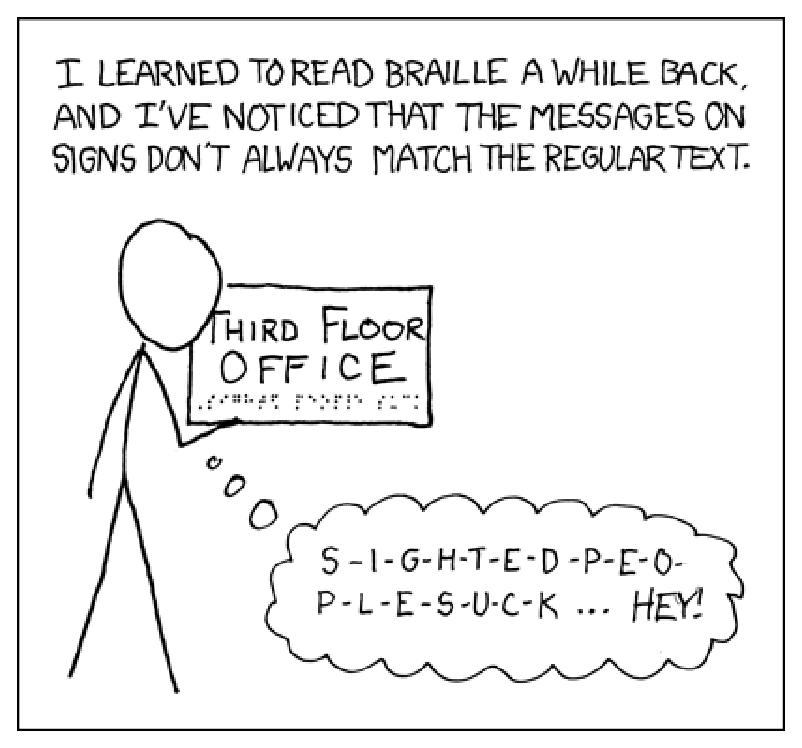
\includegraphics{../pics/braille-xkcd.eps}

(Cartoon from \url{http://xkcd.com/315/})


\myslide{Further Reading}
\MyLogo{Only if you are interested}

\begin{itemize}
\item David Samuels (2003)
  \href{https://www.tabletmag.com/sections/arts-letters/articles/chained-reader-david-samuels}{The
    Chained Reader: How the logic of machines makes us less human}
  \textit{Tablet} (accessed 2023-10-09)
\end{itemize}

% \myslide{Practice Assignment}

% \begin{itemize}
% \item Submit a text file to the digital drop box for this course
% \item Due by Friday night ()
% \item File name: test\_ID.txt (where ID is your username ID)
% \item File Content (line separated UTF-8 text):
%   \begin{itemize}
%   \item username
%   \item Languages you can write, using ISO 639-2/B codes, separated by commas
%   \item Name in roman script
%   \item Name in other scripts (as many as you want)
%   \item Finish with a newline
%   \end{itemize}
% \end{itemize}

% \myslide{Practice Assignment}
% \begin{itemize}
% \item E.g. \texttt{test\_fcbond.txt}
%   \begin{verbatim}
% fcbond
% eng, jpn
% Francis Bond 
% フランシス・ボンド
% 프란시스 본드
% \end{verbatim}
% \end{itemize}




\end{document}


%%% Local Variables: 
%%% coding: utf-8
%%% mode: latex
%%% TeX-PDF-mode: t
%%% TeX-engine: xetex
%%% End: 

